\documentclass[14pt]{report}


\usepackage[italian]{babel}
\usepackage[utf8]{inputenc}
\usepackage{graphicx}
\usepackage{enumitem}
\usepackage{amsmath}
\usepackage{physics}



\title{Appunti di Meccanica}
\author{G.Rodari}

\begin{document}

\maketitle
\tableofcontents

\chapter[Introduzione 7-3-2017]{Introduzione}

\section{La Meccanica: metodi e misure}

La meccanica é la branca della fisica che si propone di studiare i fenomeni di moto dei corpi attraverso una \emph{modellizzazione}: si riducono i corpi in gioco nel fenomeno osservato ad un sistema di punti materiali, la cui struttura e le cui relazioni sono descrivibili attraverso leggi matematiche; per situazioni particolarmente semplici parleremo di \emph{punto materiale}, un oggetto dotato di tre gradi di libertá.
Per descrivere i dati sperimentali attraverso delle leggi é necessario un confronto continuo tra risultati teorici e sperimentali, un'alternanza tra deduzione e induzione. Nello studio dei sistemi fisici si devono riconoscere le caratteristiche di un fenomeno, associate a delle \emph{grandezze fisiche}, che possono essere numericamente rappresentate una volta definita un'unitá di misura.\\ \begin{center}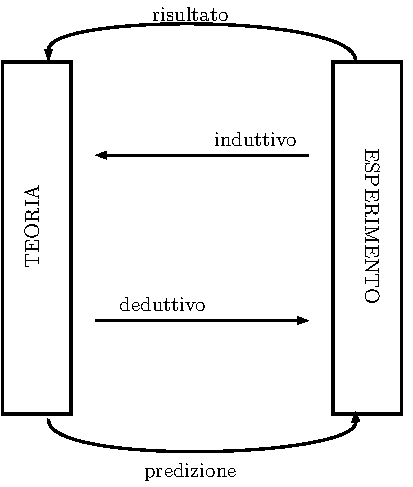
\includegraphics[scale=0.8]{tabella_metodo.pdf}\end{center}
Studiando i sistemi meccanici, ci interesserá dare risposte a due classi di problemi:
\begin{enumerate}[noitemsep]
\item Conoscendo le forze che agiscono sul sistema dedurre il moto.
\item Conoscendo il moto dei corpi dedurre le forze.
\end{enumerate}
Tutte le grandezze che entreranno in gioco possono essere derivate da tre grandezze fondamentali:
\begin{itemize}[noitemsep]
\item lunghezza $[l]$
\item tempo $[t]$
\item massa $[m]$
\end{itemize}
Ad esempio nel caso dell'energia avremo:\[[E]=[m][l]^2[t]^{-2}\]

\section{Vettori e operazioni}

Per descrivere molte grandezze sará comodo utilizzare i \emph{vettori} entitá matematiche rappresentate da un segmento orientato, dotato di:
\begin{itemize}
\item $|\vec{v}|$ modulo del vettore: ha le dimensioni della grandezza rappresentata
\item direzione: retta su cui giace il vettore
\item verso: `da che parte' va la freccina
\end{itemize}
Spesso i vettori saranno individuati dal loro punto di applicazione $Q$ e dal loro estremo libero $P$.\\IMMAGINE VETTORE
Sono definite alcune operazioni:
\subsection{Prodotto per scalare}
\[k\va{v}\]
\subsection{Somma e differenza di vettori}
\[\va{s}=\va{a}+\va{b}\]
\[\va{d}=\va{a}-\va{b}\]
\subsection{Prodotto scalare}
\[\va{a}\vdot\va{b}=\abs{\va{a}}\abs*{\va{b}}\cos\theta\]
\subsection{Prodotto vettoriale}
\[\va{a}\cp\va{b}=\abs{\va{a}}\abs*{\va{b}}\sin\theta\]
\subsection{Versore}
\[\frac{\va{v}}{\abs{\va{v}}}=\vu{u}\] si ottiene un vettore modulo 1 \textbf{adimensionale}, con la stessa direzione e lo stesso verso di $\va{v}$

\section{Riferimento cartesiano}

Per poter individuare con semplicitá un vettore é utile fissare un sistema di riferimento cartesiano, costruito considerando tre direzioni ortogonali `individuate' da versori. IMMAGINE\\
Dato un sistema di riferimento, un vettore potrá essere individuato con una terna di scalari:
\[\va{v}=(v_x, v_y, v_z)\quad\Rightarrow\quad\va{v}=v_x\vu{i}+v_y\vu{j}+v_z\vu{k}\]
In generale risulta che $\va*{v}\vdot\va*{v}=\abs{\va*{v}}^2$. Inoltre si hanno le seguenti relazioni tra versori:
\[
\left\{
\begin{array}{c}
\vu{i}\vdot\vu{i}=\vu{j}\vdot\vu{j}=\vu{k}\vdot\vu{k}=1\\
\vu{i}\vdot\vu{j}=\vu{i}\vdot\vu{k}=\vu{j}\vdot\vu{k}=0\\
\vu{i}\cp\vu{i}=\vu{j}\cp\vu{j}=\vu{k}\cp\vu{k}=0\\
\vu{i}\cp\vu{j}=\vu{k}\quad\vu{i}\cp\vu{k}=-\vu{j}\quad\vu{j}\cp\vu{k}=\vu{i}\\
\end{array}
\right.
\]

\subsection{Operazioni vettoriali in coordinate cartesiane}

In coordinate cartesiane le operazioni vettoriali possono essere scritte come:
\[\begin{split}
\va{a}+\va{b}=(a_x\vu{i}+a_y\vu{j}+a_z\vu{k})+(b_x\vu{i}+b_y\vu{j}+b_z\vu{k})=\\
=(a_x+b_x)\vu{i}+(a_y+b_y)\vu{j}+(a_z+b_z)\vu{k}
\end{split}\]
\[\begin{split}
\va{a}\vdot\va{b}=(a_x\vu{i}+a_y\vu{j}+a_z\vu{k})\vdot(b_x\vu{i}+b_y\vu{j}+b_z\vu{k})=\\
=a_xb_x+a_yb_y+a_zb_z
\end{split}\]
\[\begin{split}
\va{a}\cp\va{b}=(a_x\vu{i}+a_y\vu{j}+a_z\vu{k})\cp(b_x\vu{i}+b_y\vu{j}+b_z\vu{k})=\\
=(a_xb_y-a_yb_x)\vu{i}+(a_zb_x-a_xb_z)\vu{j}+(a_yb_z-a_zb_y)\vu{k}
\end{split}\]
In particolare il prodotto vettoriale puó essere visto come determinante della matrice:
\[
\va{a}\cp\va{b}=
\begin{vmatrix}
\vu{i} & \vu{j} & \vu{k}\\
a_x & a_y & a_z\\
b_x & b_y & b_z\\
\end{vmatrix}
\]









\end{document}